\documentclass[11pt, a4paper]{article}

\usepackage[margin=2.5cm]{geometry}
\usepackage{booktabs}
\usepackage{parskip}
\usepackage{xcolor}
\usepackage{titlesec}
\usepackage{enumitem}
\usepackage{hyperref}
\usepackage{array}
\usepackage{float}
\usepackage{amsmath}
\usepackage{graphicx}

\hypersetup{colorlinks=true, linkcolor=blue}
\titleformat{\section}{\large\bfseries}{}{0em}{}[\titlerule]
\titleformat{\subsection}{\normalsize\itshape}{}{0em}{}

\definecolor{good}{RGB}{0, 128, 0}
\definecolor{bad}{RGB}{180, 0, 0}
\definecolor{neutral}{RGB}{100, 100, 100}

\title{
    \textbf{Key Findings} \\
    \large Phase 1 — How Image Degradation Affects Stereo SLAM \\
    \normalsize EECE5554 Final Project
}
\author{Shyam Sreenivasan}
\date{\today}

\begin{document}
\maketitle

% ---------------------------------------------------------------------------
\section{Background}

We tested five types of image degradation on a stereo-inertial ORB-SLAM3 system
running on two TUM-VI room sequences (room1 and room2). Each degradation was applied
to both camera images, simulating real-world lens or sensor degradation.

Two fixed reference points were used per trajectory:

\begin{table}[H]
\centering
\begin{tabular}{lll}
\toprule
\textbf{Trajectory} & \textbf{Clean stereo ATE} & \textbf{Clean mono ATE} \\
\midrule
Dataset 1 (room1) & 0.0068 m & 0.0102 m \\
Dataset 2 (room2) & 0.0057 m & 0.0082 m \\
\bottomrule
\end{tabular}
\caption{Clean baselines for both trajectories.}
\end{table}

The mono baseline is the \textit{switching target} --- when stereo performance
degrades to this level, it is no longer worth running stereo over mono.

% ---------------------------------------------------------------------------
\section{Finding 1 — Each Degradation Type Has a Unique Failure Signature}

\subsection{Dataset 1 (room1)}

\begin{table}[H]
\centering
\begin{tabular}{lllll}
\toprule
\textbf{Type} & \textbf{Parameter} & \textbf{Failure at} & \textbf{ATE just before cliff} & \textbf{Shape} \\
\midrule
Gaussian blur   & sigma ($\sigma$)      & $\sigma = 6.1$    & 0.0102 m (+50\%)  & Gradual \\
Motion blur     & kernel length         & 28 pixels         & 0.0170 m (+150\%) & Steep \\
Salt \& pepper  & pixel density         & 40\%              & 0.0074 m (+9\%)   & Flat then cliff \\
Brightness      & scale factor $\alpha$ & $\alpha = 0.03$   & 0.0098 m (+44\%)  & Asymmetric \\
Occlusion       & fraction blocked      & 61\%              & 0.0086 m (+26\%)  & Flat then cliff \\
\bottomrule
\end{tabular}
\caption{Failure thresholds and degradation shape for room1.}
\end{table}

\subsection{Dataset 2 (room2)}

\begin{table}[H]
\centering
\begin{tabular}{lllll}
\toprule
\textbf{Type} & \textbf{Parameter} & \textbf{Failure at} & \textbf{ATE just before cliff} & \textbf{Shape} \\
\midrule
Gaussian blur   & sigma ($\sigma$)      & $\sigma = 6.0$    & 0.0075 m (+31\%)  & Gradual \\
Motion blur     & kernel length         & 27 pixels         & 0.0085 m (+49\%)  & Steep \\
Salt \& pepper  & pixel density         & 40\%              & 0.0074 m (+30\%)  & Flat then cliff \\
Brightness      & scale factor $\alpha$ & $\alpha = 0.02$   & 0.0063 m (+10\%)  & Asymmetric \\
Occlusion       & fraction blocked      & 61\%              & 0.0073 m (+28\%)  & Flat then cliff \\
\bottomrule
\end{tabular}
\caption{Failure thresholds and degradation shape for room2.}
\end{table}

Not all degradations are equally dangerous or equally detectable. Failure thresholds
are scene-dependent but the overall pattern is consistent across both datasets.

\begin{figure}[H]
    \centering
    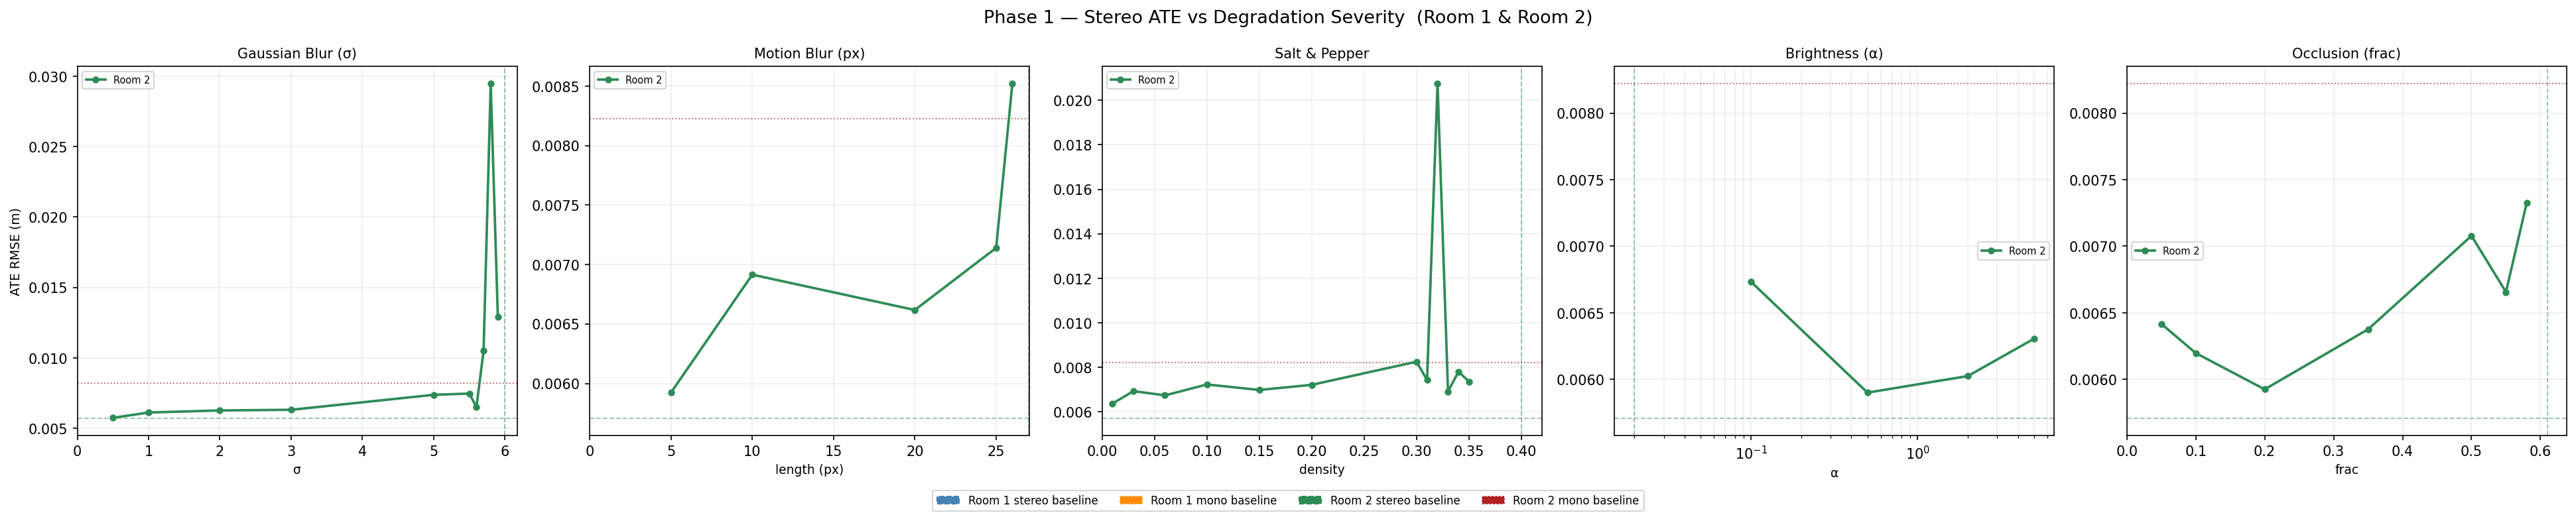
\includegraphics[width=\textwidth]{phase1_combined.png}
    \caption{Combined Phase 1 sweep results for all 5 degradation types across Room 1 (blue) and Room 2 (green).
             Dashed lines = stereo baselines; dotted lines = mono baselines.
             Vertical dashed lines mark the failure cliff for each trajectory.}
\end{figure}

% ---------------------------------------------------------------------------
\section{Finding 2 — The Mono Baseline is a Natural Switching Point}

As degradation increases, stereo ATE rises until it meets the mono baseline ---
and then SLAM fails. This is not a coincidence.

Stereo SLAM's advantage over mono comes from metric depth via the stereo baseline.
As cameras degrade, stereo matching becomes unreliable, the depth anchor is lost,
and the system effectively falls back to behaving like mono. One more step of
degradation and tracking fails entirely.

\textbf{The crossover point is therefore both a natural and physically meaningful
switching threshold}: below it, stereo is earning its advantage; at it, stereo
has lost its advantage; beyond it, stereo has failed outright.

\subsection{Dataset 1 (room1)}
\begin{itemize}
    \item Gaussian blur: crossover at $\sigma = 6.0$ (ATE = 0.0102 m, exactly at mono baseline)
    \item Motion blur: crossover at length = 25 px (ATE = 0.0170 m, well above mono baseline)
\end{itemize}

\subsection{Dataset 2 (room2)}
\begin{itemize}
    \item Gaussian blur: crossover at $\sigma = 5.7$ (ATE = 0.0105 m, just above mono baseline)
    \item Motion blur: crossover at length = 26 px (ATE = 0.0085 m, just above mono baseline)
\end{itemize}

\begin{figure}[H]
    \centering
    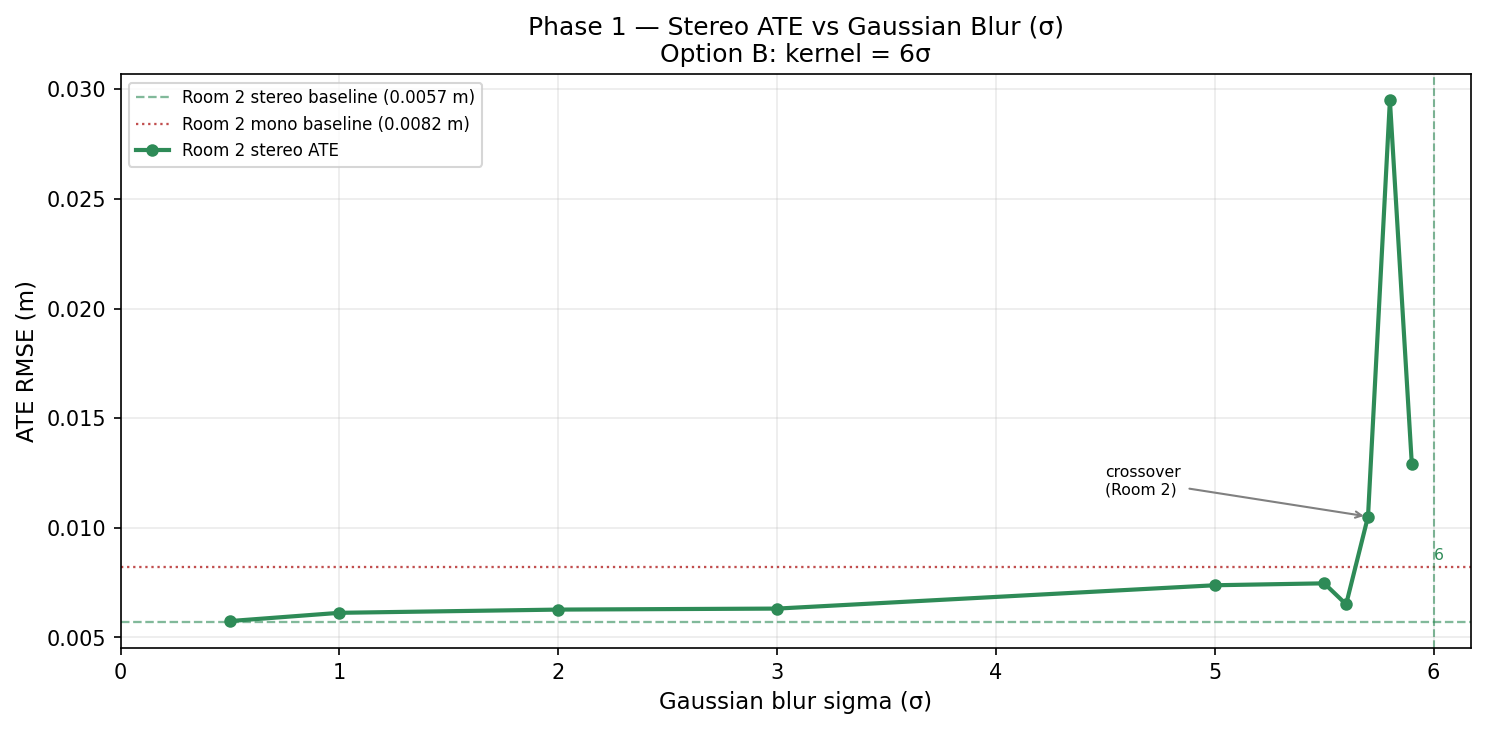
\includegraphics[width=0.49\textwidth]{phase1_blur.png}
    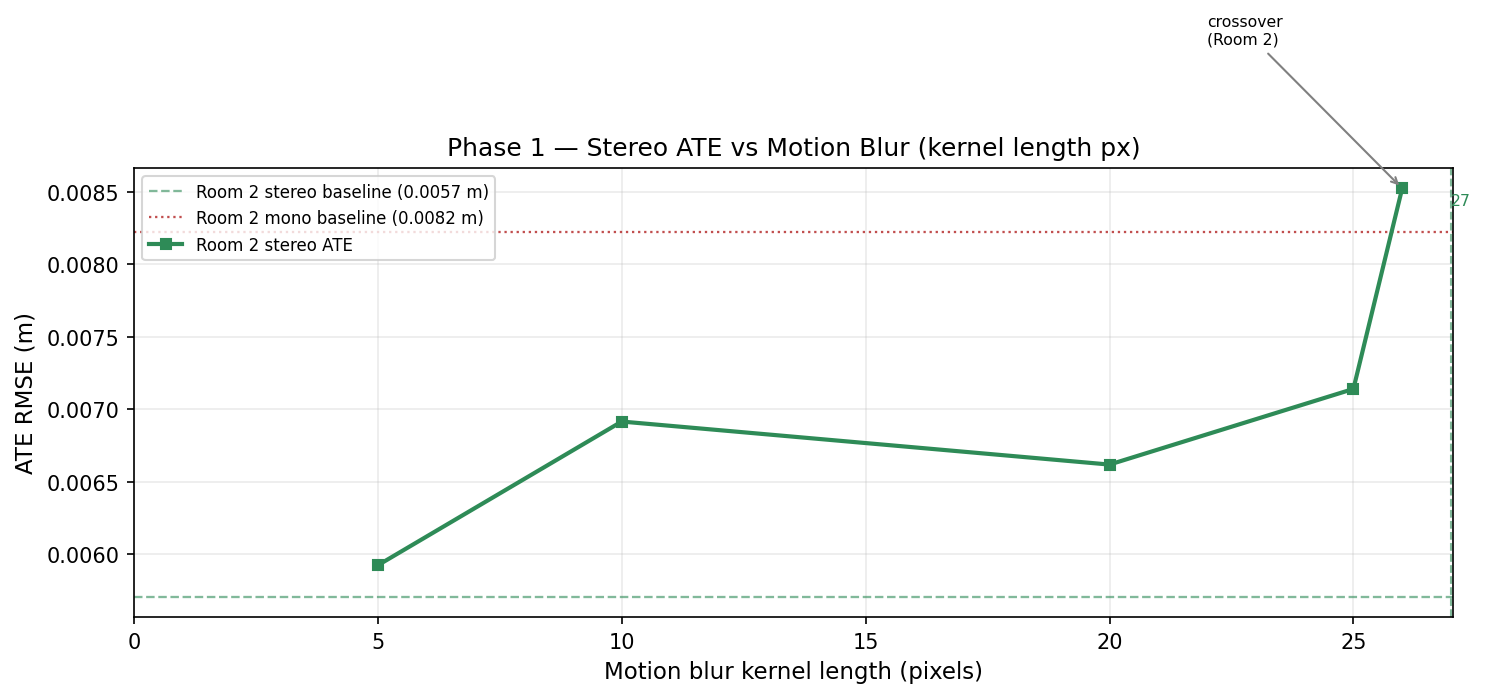
\includegraphics[width=0.49\textwidth]{phase1_motion_blur.png}
    \caption{Gaussian blur (left) and motion blur (right) — gradual ATE curves with visible crossover before failure.}
\end{figure}

This validates the health monitor's severity metric:
$$\text{severity} = \frac{\text{RTE}_{\text{stereo}}}{\text{RTE}_{\text{stereo}} + \text{RTE}_{\text{mono}}}$$
The crossover at severity = 0.5 is the correct trigger point.

% ---------------------------------------------------------------------------
\section{Finding 3 — ORB-SLAM3 is Robust to Random Pixel Corruption}

Salt \& pepper noise and occlusion both showed a \textbf{flat ATE curve} across
most of their range:

\subsection{Dataset 1 (room1)}
\begin{itemize}
    \item Salt \& pepper: ATE barely changes from 1\% up to 35\% corrupted pixels
    \item Occlusion: ATE barely changes from 5\% up to 58\% of image blocked
\end{itemize}

\subsection{Dataset 2 (room2)}
\begin{itemize}
    \item Salt \& pepper: ATE stays 0.0064--0.0083 m from 1\% up to 35\% corrupted pixels
    \item Occlusion: ATE stays 0.0059--0.0073 m from 5\% up to 58\% of image blocked
\end{itemize}

The reason is ORB-SLAM3's built-in outlier rejection (RANSAC). Random corrupted
pixels or a contiguous blocked region look like outlier keypoints, which RANSAC
discards automatically. SLAM only fails when so much of the image is corrupted
that there are not enough good keypoints left to track.

\textbf{Implication:} These degradations produce no learnable gradient for the
health monitor. The signal is binary (fine, then suddenly failed) with no
warning zone.

\begin{figure}[H]
    \centering
    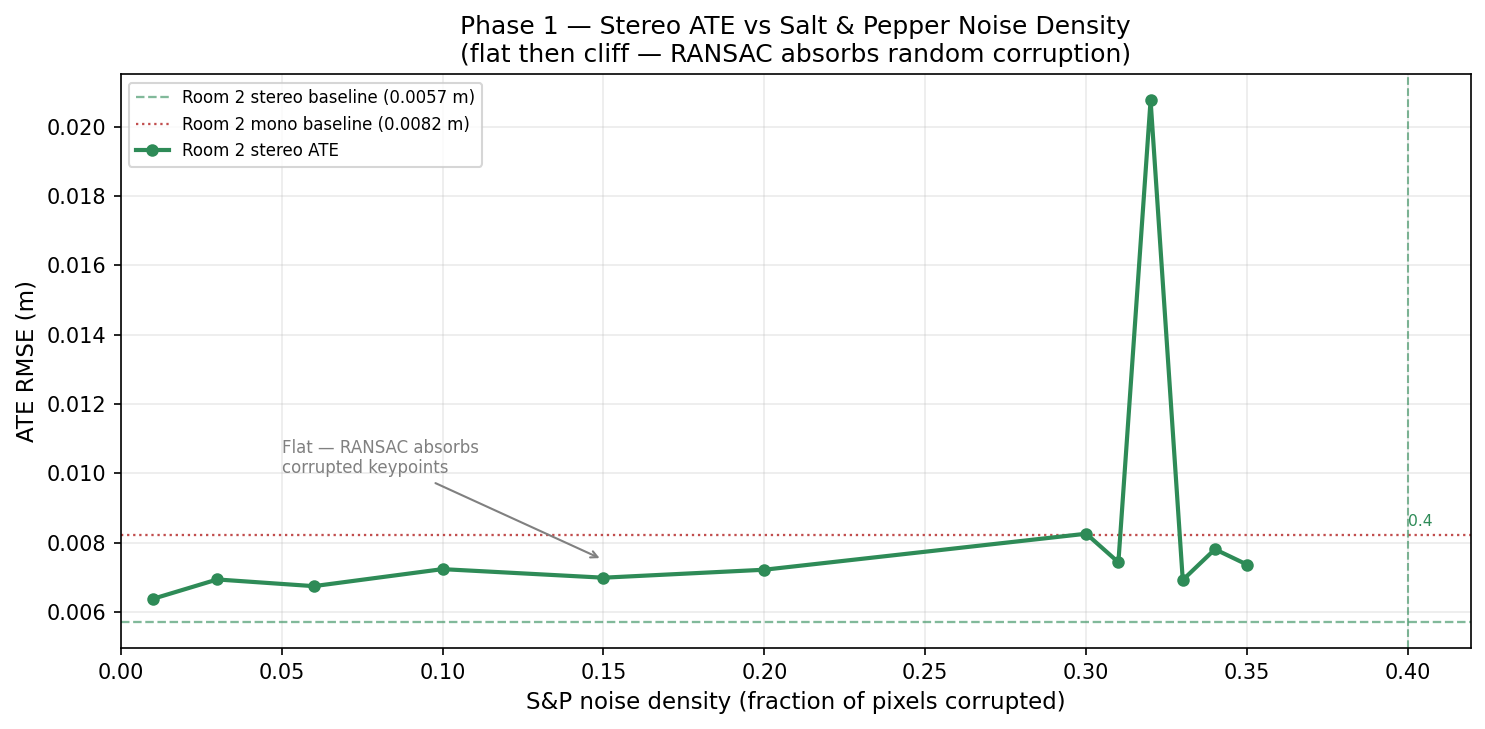
\includegraphics[width=0.49\textwidth]{phase1_snp.png}
    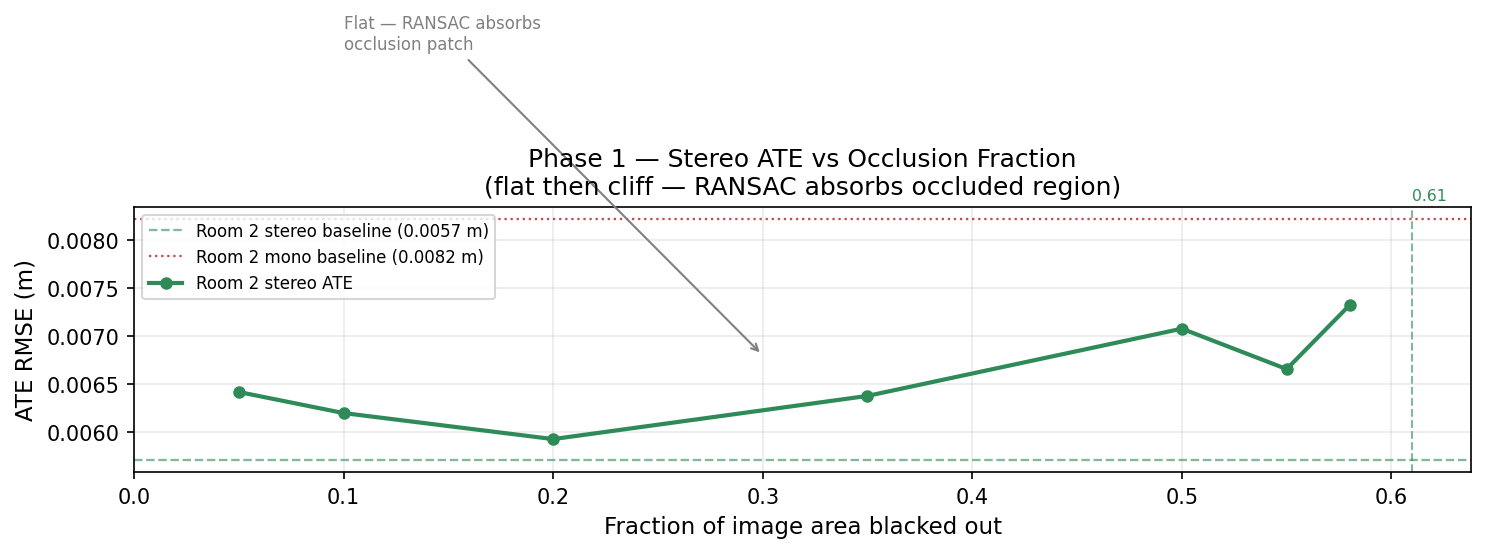
\includegraphics[width=0.49\textwidth]{phase1_occlusion.png}
    \caption{Salt \& pepper (left) and occlusion (right) — flat ATE curves followed by a hard cliff.}
\end{figure}

% ---------------------------------------------------------------------------
\section{Finding 4 — Underexposure is Far More Dangerous Than Overexposure}

Brightness degradation is strongly asymmetric:

\subsection{Dataset 1 (room1)}
\begin{itemize}
    \item \textbf{Overexposure} up to $10\times$ normal brightness: SLAM survives, ATE only 22\% worse
    \item \textbf{Underexposure} below $\alpha = 0.03$: SLAM fails immediately
\end{itemize}

\subsection{Dataset 2 (room2)}
\begin{itemize}
    \item \textbf{Overexposure} up to $5\times$ normal brightness: SLAM survives, ATE only 10\% worse
    \item \textbf{Underexposure} below $\alpha = 0.02$: SLAM fails immediately
\end{itemize}

The reason: ORB feature detection relies on intensity gradients (edges and corners).
In very dark images, all pixel values collapse toward zero and gradients disappear.
In bright (overexposed) images, gradients still exist at object boundaries even
when highlights are clipped.

\textbf{Implication:} A simple brightness check (mean pixel intensity below a
threshold) could detect extreme underexposure without needing a neural network.

\begin{figure}[H]
    \centering
    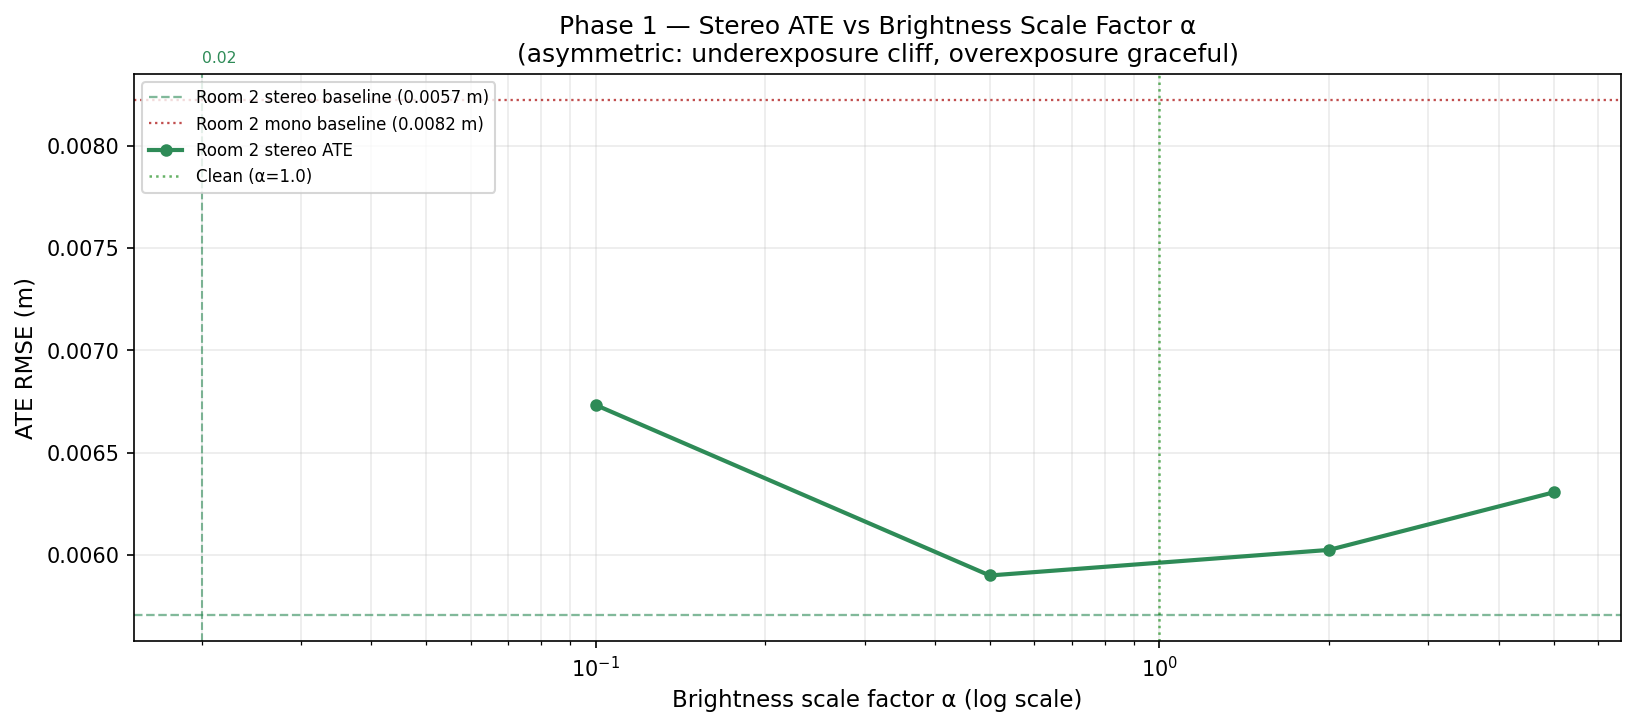
\includegraphics[width=0.65\textwidth]{phase1_brightness.png}
    \caption{Brightness sweep — asymmetric response: overexposure is benign, underexposure causes immediate failure.}
\end{figure}

% ---------------------------------------------------------------------------
\section{Finding 5 — Gaussian Blur and Motion Blur are the Best Candidates for Health Monitoring}

These two degradations produce a \textbf{gradual, learnable severity curve}:

\subsection{Dataset 1 (room1)}

\textbf{Gaussian blur:}
\begin{itemize}
    \item ATE rises steadily from clean (+1.5\%) to crossover (+50\%) over 7 sigma levels
    \item Long warning window before failure at $\sigma = 6.1$
\end{itemize}

\textbf{Motion blur:}
\begin{itemize}
    \item ATE rises steeply --- +150\% just before failure at length = 28 px
    \item Shorter warning window but very strong signal
\end{itemize}

\subsection{Dataset 2 (room2)}

\textbf{Gaussian blur:}
\begin{itemize}
    \item ATE rises from clean (+1\%) to crossover (+84\%) across 7 sigma levels
    \item Cliff is slightly earlier ($\sigma = 6.0$) than room1, reflecting scene texture differences
\end{itemize}

\textbf{Motion blur:}
\begin{itemize}
    \item ATE rises from clean to crossover at length = 26 px (just above mono baseline)
    \item Cliff is one pixel step later than room1 (27 vs 28 px), consistent behavior
\end{itemize}

Both types give the health monitor a continuous input-output relationship to
learn: as images get blurrier, severity increases monotonically. This is exactly
what a regression model needs.

% ---------------------------------------------------------------------------
\section{Finding 6 — The Cliff is Sharp and Scene-Dependent}

Across all degradation types, once SLAM fails at a given severity level, every
higher level also fails. There is no recovery.

\subsection{Dataset 1 (room1)}
The transition zone is typically one parameter step wide:
$\sigma = 6.0$ succeeds, $\sigma = 6.1$ fails.

\subsection{Dataset 2 (room2)}
Similarly sharp transitions: $\sigma = 5.9$ succeeds, $\sigma = 6.0$ fails.
Motion blur fails at length = 27 px vs. room1's 28 px.

The exact threshold varies by scene (texture density, lighting, scene depth),
but the cliff pattern is consistent: success up to a hard limit, then total failure.

This has two implications:
\begin{enumerate}
    \item The health monitor must act \textit{before} the cliff, not at it
    \item There is no benefit to running stereo once the cliff is crossed ---
          immediate switch to mono is the right policy
\end{enumerate}

% ---------------------------------------------------------------------------
\section{Generalised Inference}

The following conclusions hold across both datasets:

\begin{enumerate}
    \item \textbf{Blur (Gaussian and motion) is the most informative degradation type.}
          Both produce a monotonically increasing ATE curve that crosses the mono
          baseline before SLAM fails --- giving the health monitor a clear, learnable
          signal with a meaningful warning window.

    \item \textbf{Random corruption (S\&P, occlusion) is absorbed by RANSAC.}
          ATE stays flat across a wide severity range, then collapses in one step.
          No warning zone exists, making these poor health monitor targets.

    \item \textbf{Brightness has an asymmetric response.}
          Overexposure is benign; underexposure is catastrophic. A simple rule-based
          check is sufficient --- no learned model needed.

    \item \textbf{Failure thresholds are scene-dependent but patterns are not.}
          Room2 fails at slightly lower blur than room1, but both show the same
          crossover-then-cliff structure. A model trained across multiple scenes
          will generalise better than one trained on a single trajectory.

    \item \textbf{The mono baseline crossover is a universal switching anchor.}
          In both trajectories, the point where stereo ATE equals mono ATE corresponds
          to the last stable operating point before SLAM failure. This makes
          severity $= 0.5$ a physically grounded and scene-agnostic trigger threshold.
\end{enumerate}

% ---------------------------------------------------------------------------
\section{Recommendation for Phase 2}

Based on these findings, Phase 2 (health monitor training) should:

\begin{enumerate}
    \item \textbf{Focus training data on Gaussian blur and motion blur} ---
          these provide the richest severity gradients across both trajectories
    \item \textbf{Use data from both trajectories} ---
          room1 and room2 differ in texture and lighting, increasing model generalisation
    \item \textbf{Use the mono baseline crossover as the severity=1 anchor} ---
          already implemented via the ratio policy
    \item \textbf{Target early detection} --- the model should predict high severity
          one or two steps before the cliff, not at the cliff itself
    \item \textbf{Consider salt \& pepper and occlusion as hard negatives} ---
          the model should learn to output low severity for these even at
          high degradation levels, since SLAM is unaffected
\end{enumerate}

\end{document}
